\section{eo\-Rng Class Reference}
\label{classeo_rng}\index{eoRng@{eoRng}}
Random Number Generator.  


{\tt \#include $<$utils/eo\-RNG.h$>$}

Inheritance diagram for eo\-Rng::\begin{figure}[H]
\begin{center}
\leavevmode
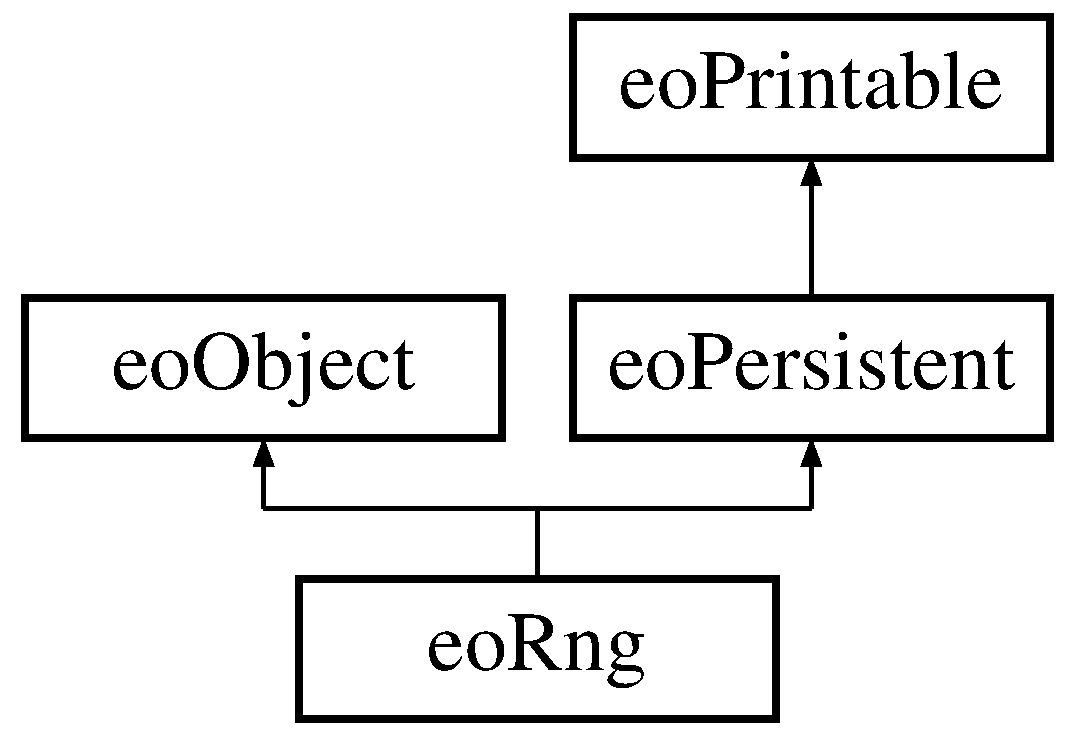
\includegraphics[height=3cm]{classeo_rng}
\end{center}
\end{figure}
\subsection*{Public Member Functions}
\begin{CompactItemize}
\item 
{\bf eo\-Rng} (uint32\_\-t s)
\begin{CompactList}\small\item\em Constructor. \item\end{CompactList}\item 
void {\bf reseed} (uint32\_\-t s)
\begin{CompactList}\small\item\em Re-initializes the Random Number Generator. \item\end{CompactList}\item 
void {\bf old\-Reseed} (uint32\_\-t s)
\begin{CompactList}\small\item\em Re-initializes the Random Number Generator. \item\end{CompactList}\item 
double {\bf uniform} (double m=1.0)\label{classeo_rng_a4}

\begin{CompactList}\small\item\em uniform(m = 1.0) returns a random double in the range [0, m) \item\end{CompactList}\item 
uint32\_\-t {\bf random} (uint32\_\-t m)\label{classeo_rng_a5}

\begin{CompactList}\small\item\em {\bf random()}{\rm (p.\,\pageref{classeo_rng_a5})} returns a random integer in the range [0, m) \item\end{CompactList}\item 
bool {\bf flip} (float bias=0.5)\label{classeo_rng_a6}

\begin{CompactList}\small\item\em {\bf flip()}{\rm (p.\,\pageref{classeo_rng_a6})} tosses a biased coin such that flip(x/100.0) will returns true x\% of the time \item\end{CompactList}\item 
double {\bf normal} (void)\label{classeo_rng_a7}

\begin{CompactList}\small\item\em {\bf normal()}{\rm (p.\,\pageref{classeo_rng_a7})} zero mean gaussian deviate with standard deviation of 1 \item\end{CompactList}\item 
double {\bf normal} (double stdev)\label{classeo_rng_a8}

\begin{CompactList}\small\item\em normal(stdev) zero mean gaussian deviate with user defined standard deviation \item\end{CompactList}\item 
double {\bf normal} (double mean, double stdev)\label{classeo_rng_a9}

\begin{CompactList}\small\item\em normal(mean, stdev) user defined mean gaussian deviate with user defined standard deviation \item\end{CompactList}\item 
double {\bf negexp} (double mean)\label{classeo_rng_a10}

\begin{CompactList}\small\item\em Generates random numbers using a negative exponential distribution. \item\end{CompactList}\item 
uint32\_\-t {\bf rand} ()\label{classeo_rng_a11}

\begin{CompactList}\small\item\em {\bf rand()}{\rm (p.\,\pageref{classeo_rng_a11})} returns a random number in the range [0, rand\_\-max) \item\end{CompactList}\item 
uint32\_\-t {\bf rand\_\-max} (void) const \label{classeo_rng_a12}

\begin{CompactList}\small\item\em {\bf rand\_\-max()}{\rm (p.\,\pageref{classeo_rng_a12})} the maximum returned by {\bf rand()}{\rm (p.\,\pageref{classeo_rng_a11})} \item\end{CompactList}\item 
template$<$typename TYPE$>$ int {\bf roulette\_\-wheel} (const std::vector$<$ TYPE $>$ \&vec, TYPE total=0)
\begin{CompactList}\small\item\em roulette\_\-wheel(vec, total = 0) does a roulette wheel selection on the input std::vector vec. \item\end{CompactList}\item 
template$<$typename TYPE$>$ const TYPE \& {\bf choice} (const std::vector$<$ TYPE $>$ \&vec) const 
\begin{CompactList}\small\item\em Randomly select element from vector. \item\end{CompactList}\item 
template$<$typename TYPE$>$ TYPE \& {\bf choice} (std::vector$<$ TYPE $>$ \&vec)
\begin{CompactList}\small\item\em Randomly select element from vector. \item\end{CompactList}\item 
void {\bf print\-On} (std::ostream \&\_\-os) const 
\begin{CompactList}\small\item\em Write object. \item\end{CompactList}\item 
void {\bf read\-From} (std::istream \&\_\-is)
\begin{CompactList}\small\item\em Read object. \item\end{CompactList}\item 
std::string {\bf class\-Name} (void) const 
\begin{CompactList}\small\item\em Return the class id. \item\end{CompactList}\end{CompactItemize}
\subsection*{Private Member Functions}
\begin{CompactItemize}
\item 
uint32\_\-t {\bf restart} (void)\label{classeo_rng_d0}

\item 
void {\bf initialize} (uint32\_\-t seed)\label{classeo_rng_d1}

\item 
{\bf eo\-Rng} (const {\bf eo\-Rng} \&)
\begin{CompactList}\small\item\em Copy constructor. \item\end{CompactList}\item 
{\bf eo\-Rng} \& {\bf operator=} (const {\bf eo\-Rng} \&)
\begin{CompactList}\small\item\em Assignmant operator. \item\end{CompactList}\end{CompactItemize}
\subsection*{Private Attributes}
\begin{CompactItemize}
\item 
uint32\_\-t $\ast$ {\bf state}\label{classeo_rng_r0}

\begin{CompactList}\small\item\em Array for the state. \item\end{CompactList}\item 
uint32\_\-t $\ast$ {\bf next}\label{classeo_rng_r1}

\item 
int {\bf left}\label{classeo_rng_r2}

\item 
bool {\bf cached}\label{classeo_rng_r3}

\item 
float {\bf cache\-Value}\label{classeo_rng_r4}

\item 
const int {\bf N}\label{classeo_rng_r5}

\item 
const int {\bf M}\label{classeo_rng_r6}

\item 
const uint32\_\-t {\bf K}\label{classeo_rng_r7}

\begin{CompactList}\small\item\em Magic constant. \item\end{CompactList}\end{CompactItemize}


\subsection{Detailed Description}
Random Number Generator. 

eo\-Rng is a persistent class that uses the ``Mersenne Twister'' random number generator MT19937 for generating random numbers. The various member functions implement useful functions for evolutionary algorithms. Included are: {\bf rand()}{\rm (p.\,\pageref{classeo_rng_a11})}, {\bf random()}{\rm (p.\,\pageref{classeo_rng_a5})}, {\bf flip()}{\rm (p.\,\pageref{classeo_rng_a6})} and {\bf normal()}{\rm (p.\,\pageref{classeo_rng_a7})}.

{\bf EO}{\rm (p.\,\pageref{class_e_o})} provides a global random number generator {\tt rng} that is seeded by the current UNIX time at program start. Moreover some global convenience functions are provided that use the global random number generator: {\tt random}, {\tt normal}.

\begin{Desc}
\item[Warning:]If you want to repeatedly generated the same sequence of pseudo-random numbers, you should always reseed the generator at the beginning of your code.\end{Desc}
\subsection*{Documentation in original file}

This is the ``Mersenne Twister'' random number generator MT19937, which generates pseudorandom integers uniformly distributed in 0..(2$^\wedge$32 - 1) starting from any odd seed in 0..(2$^\wedge$32 - 1). This version is a recode by Shawn Cokus ({\tt Cokus@math.washington.edu}) on March 8, 1998 of a version by Takuji Nishimura (who had suggestions from Topher Cooper and Marc Rieffel in July-August 1997).

Effectiveness of the recoding (on Goedel2.math.washington.edu, a DEC Alpha running OSF/1) using GCC -O3 as a compiler: before recoding: 51.6 sec. to generate 300 million random numbers; after recoding: 24.0 sec. for the same (i.e., 46.5\% of original time), so speed is now about 12.5 million random number generations per second on this machine.

According to the URL $<${\tt http://www.math.keio.ac.jp/$\sim$matumoto/emt.html}$>$ (and paraphrasing a bit in places), the Mersenne Twister is ``designed with consideration of the flaws of various existing generators,'' has a period of 2$^\wedge$19937 - 1, gives a sequence that is 623-dimensionally equidistributed, and ``has passed many std::stringent tests, including the die-hard test of G. Marsaglia and the load test of P. Hellekalek and S. Wegenkittl.'' It is efficient in memory usage (typically using 2506 to 5012 bytes of static data, depending on data type sizes, and the code is quite short as well). It generates random numbers in batches of 624 at a time, so the caching and pipelining of modern systems is exploited. It is also divide- and mod-free.

The code as Shawn received it included the following notice: {\tt Copyright (C) 1997 Makoto Matsumoto and Takuji Nishimura. When you use this, send an e-mail to $<${\tt matumoto@math.keio.ac.jp}$>$ with an appropriate reference to your work.} It would be nice to Cc: $<${\tt Cokus@math.washington.edu}$>$ and $<${\tt eodev-main@lists.sourceforge.net}$>$ when you write.

\subsection*{Portability}

Note for people porting {\bf EO}{\rm (p.\,\pageref{class_e_o})} to other platforms: please make sure that the type uint32\_\-t in the file {\bf eo\-Rng.h}{\rm (p.\,\pageref{eo_r_n_g_8h})} is exactly 32 bits long. It may in principle be longer, but not shorter. If it is longer, file compatibility between {\bf EO}{\rm (p.\,\pageref{class_e_o})} on different platforms may be broken. 



Definition at line 103 of file eo\-RNG.h.

\subsection{Constructor \& Destructor Documentation}
\index{eoRng@{eo\-Rng}!eoRng@{eoRng}}
\index{eoRng@{eoRng}!eoRng@{eo\-Rng}}
\subsubsection{\setlength{\rightskip}{0pt plus 5cm}eo\-Rng::eo\-Rng (uint32\_\-t {\em s})\hspace{0.3cm}{\tt  [inline]}}\label{classeo_rng_a0}


Constructor. 

\begin{Desc}
\item[Parameters:]
\begin{description}
\item[{\em s}]Random seed; if you want another seed, use reseed.\end{description}
\end{Desc}
\begin{Desc}
\item[See also:]{\bf reseed}{\rm (p.\,\pageref{classeo_rng_a2})} for details on usage of the seeding value. \end{Desc}


Definition at line 113 of file eo\-RNG.h.

References K, and state.\index{eoRng@{eo\-Rng}!eoRng@{eoRng}}
\index{eoRng@{eoRng}!eoRng@{eo\-Rng}}
\subsubsection{\setlength{\rightskip}{0pt plus 5cm}eo\-Rng::eo\-Rng (const {\bf eo\-Rng} \&)\hspace{0.3cm}{\tt  [private]}}\label{classeo_rng_d2}


Copy constructor. 

Private copy ctor and assignment operator to make sure that nobody accidentally copies the random number generator. If you want similar RNG's, make two RNG's and initialize them with the same seed.

As it cannot be called, we do not provide an implementation. 

\subsection{Member Function Documentation}
\index{eoRng@{eo\-Rng}!reseed@{reseed}}
\index{reseed@{reseed}!eoRng@{eo\-Rng}}
\subsubsection{\setlength{\rightskip}{0pt plus 5cm}void eo\-Rng::reseed (uint32\_\-t {\em s})\hspace{0.3cm}{\tt  [inline]}}\label{classeo_rng_a2}


Re-initializes the Random Number Generator. 

WARNING: Jeroen Eggermont $<${\tt jeggermo@liacs.nl}$>$ noticed that initialize does not differentiate between odd and even numbers, therefore the argument to reseed is now doubled before being passed on.

Manually divide the seed by 2 if you want to re-run old runs

\begin{Desc}
\item[Version:]MS. 5 Oct. 2001 \end{Desc}


Definition at line 135 of file eo\-RNG.h.\index{eoRng@{eo\-Rng}!oldReseed@{oldReseed}}
\index{oldReseed@{oldReseed}!eoRng@{eo\-Rng}}
\subsubsection{\setlength{\rightskip}{0pt plus 5cm}void eo\-Rng::old\-Reseed (uint32\_\-t {\em s})\hspace{0.3cm}{\tt  [inline]}}\label{classeo_rng_a3}


Re-initializes the Random Number Generator. 

This is the traditional seeding procedure. This version is deprecated and only provided for compatibility with old code. In new projects you should use reseed.

\begin{Desc}
\item[See also:]{\bf reseed}{\rm (p.\,\pageref{classeo_rng_a2})} for details on usage of the seeding value.\end{Desc}
\begin{Desc}
\item[Version:]old version (deprecated) \end{Desc}


Definition at line 150 of file eo\-RNG.h.\index{eoRng@{eo\-Rng}!roulette_wheel@{roulette\_\-wheel}}
\index{roulette_wheel@{roulette\_\-wheel}!eoRng@{eo\-Rng}}
\subsubsection{\setlength{\rightskip}{0pt plus 5cm}template$<$typename TYPE$>$ int eo\-Rng::roulette\_\-wheel (const std::vector$<$ TYPE $>$ \& {\em vec}, TYPE {\em total} = {\tt 0})\hspace{0.3cm}{\tt  [inline]}}\label{classeo_rng_a13}


roulette\_\-wheel(vec, total = 0) does a roulette wheel selection on the input std::vector vec. 

If the total is not supplied, it is calculated. It returns an integer denoting the selected argument. 

Definition at line 225 of file eo\-RNG.h.

References uniform().

Referenced by eo\-Prop\-Combined\-Quad\-Op$<$ EOT $>$::operator()(), eo\-Prop\-Combined\-Bin\-Op$<$ EOT $>$::operator()(), eo\-Prop\-Combined\-Mon\-Op$<$ EOT $>$::operator()(), and eo\-Combined\-Init$<$ EOT $>$::operator()().\index{eoRng@{eo\-Rng}!choice@{choice}}
\index{choice@{choice}!eoRng@{eo\-Rng}}
\subsubsection{\setlength{\rightskip}{0pt plus 5cm}template$<$typename TYPE$>$ const TYPE\& eo\-Rng::choice (const std::vector$<$ TYPE $>$ \& {\em vec}) const\hspace{0.3cm}{\tt  [inline]}}\label{classeo_rng_a14}


Randomly select element from vector. 

\begin{Desc}
\item[Returns:]Uniformly chosen element from the vector. \end{Desc}


Definition at line 247 of file eo\-RNG.h.

References random().\index{eoRng@{eo\-Rng}!choice@{choice}}
\index{choice@{choice}!eoRng@{eo\-Rng}}
\subsubsection{\setlength{\rightskip}{0pt plus 5cm}template$<$typename TYPE$>$ TYPE\& eo\-Rng::choice (std::vector$<$ TYPE $>$ \& {\em vec})\hspace{0.3cm}{\tt  [inline]}}\label{classeo_rng_a15}


Randomly select element from vector. 

This is an overloaded member function, provided for convenience. It differs from the above function only in what argument(s) it accepts.

Provide a version returning a non-const element reference.

\begin{Desc}
\item[Returns:]Uniformly chosen element from the vector.\end{Desc}
\begin{Desc}
\item[Warning:]Changing the return value does alter the vector. \end{Desc}


Definition at line 262 of file eo\-RNG.h.

References random().\index{eoRng@{eo\-Rng}!printOn@{printOn}}
\index{printOn@{printOn}!eoRng@{eo\-Rng}}
\subsubsection{\setlength{\rightskip}{0pt plus 5cm}void eo\-Rng::print\-On (std::ostream \& {\em \_\-os}) const\hspace{0.3cm}{\tt  [inline, virtual]}}\label{classeo_rng_a16}


Write object. 

It's called print\-On since it prints the object on a stream. \begin{Desc}
\item[Parameters:]
\begin{description}
\item[{\em \_\-os}]A std::ostream. \end{description}
\end{Desc}


Implements {\bf eo\-Printable} {\rm (p.\,\pageref{classeo_printable_a1})}.

Definition at line 266 of file eo\-RNG.h.

References state.\index{eoRng@{eo\-Rng}!readFrom@{readFrom}}
\index{readFrom@{readFrom}!eoRng@{eo\-Rng}}
\subsubsection{\setlength{\rightskip}{0pt plus 5cm}void eo\-Rng::read\-From (std::istream \& {\em \_\-is})\hspace{0.3cm}{\tt  [inline, virtual]}}\label{classeo_rng_a17}


Read object. 

\begin{Desc}
\item[Parameters:]
\begin{description}
\item[{\em \_\-is}]A std::istream. \end{description}
\end{Desc}
\begin{Desc}
\item[Exceptions:]
\begin{description}
\item[{\em runtime\_\-std::exception}]If a valid object can't be read. \end{description}
\end{Desc}


Implements {\bf eo\-Persistent} {\rm (p.\,\pageref{classeo_persistent_a1})}.

Definition at line 277 of file eo\-RNG.h.

References state.\index{eoRng@{eo\-Rng}!className@{className}}
\index{className@{className}!eoRng@{eo\-Rng}}
\subsubsection{\setlength{\rightskip}{0pt plus 5cm}std::string eo\-Rng::class\-Name (void) const\hspace{0.3cm}{\tt  [inline, virtual]}}\label{classeo_rng_a18}


Return the class id. 

This should be redefined in each class. Only \char`\"{}leaf\char`\"{} classes can be non-virtual.

Maarten: removed the default implementation as this proved to be too error-prone: I found several classes that had a typo in class\-Name (like classname), which would print {\bf eo\-Object}{\rm (p.\,\pageref{classeo_object})} instead of their own. Having it pure will force the implementor to provide a name. 

Implements {\bf eo\-Object} {\rm (p.\,\pageref{classeo_object_a1})}.

Definition at line 293 of file eo\-RNG.h.\index{eoRng@{eo\-Rng}!operator=@{operator=}}
\index{operator=@{operator=}!eoRng@{eo\-Rng}}
\subsubsection{\setlength{\rightskip}{0pt plus 5cm}{\bf eo\-Rng}\& eo\-Rng::operator= (const {\bf eo\-Rng} \&)\hspace{0.3cm}{\tt  [private]}}\label{classeo_rng_d3}


Assignmant operator. 

\begin{Desc}
\item[See also:]Copy constructor {\bf eo\-Rng(const eo\-Rng\&)}{\rm (p.\,\pageref{classeo_rng_d2})}. \end{Desc}


The documentation for this class was generated from the following file:\begin{CompactItemize}
\item 
eo\-RNG.h\end{CompactItemize}
